\subsection{Pitch Generation}\label{subsec:Pitch_Generation}

Die Hauptaufgabe der Komponente Pitch Generation ist es das Audiosignal aus dem Rechtecksignal der Tonhöhenantenne (Pitch Antenna) zu generieren. Pitch Generation nimmt zudem eine Frequenzmessung des Audiosignals vor um diverse Funktionalitäten zu gewährleisten. In Abbildung \ref{img:Blockschaltbild_pitch} ist der Grobe aufbau der Komponente aufgezeigt. Die genaue Erklärung zu den einzelnen Komponenten ist in den folgenden Abschnitten zu finden.


\begin{figure}[h!]
	\centering
	\includegraphics[width=1\textwidth]{Blockschaltbild_pitch.pdf}
	\caption{Blockschaltbild der Custom IP Pitch Generation} 
	\label{img:Blockschaltbild_pitch}
\end{figure}  



\paragraph{Referenzoszillator}

Der Referenzoszillator ist wie in Kapitel ... \todo{Referenz auf Grundlagen digitales Theremin} dafür zuständig ein Sinussignal mit Einer Frequenz ähnlich wie der Antennenoszillator ui generieren. Er generiert diesen wie schon erwähnt mithilfe des Cordic Algorithmus. Er ist aufgeteilt in zwei Komponenten: der Cordic Controller und der Cordic Processor. Wie diese beiden Komponenten miteinander verbunden sind ist in Abbildung \ref{img:Referenceoscillator} ersichtlich. \\

Der Cordic Controller berechnet den Winkelwert phi in der Form von Abbildung ... \todo{referenz Bild phi einfügen}

\begin{figure}[h!]
	\centering
	
\includegraphics[width=0.53\textwidth]{Referenceoscillator.pdf}
	\caption{Aufbau des Referenzoszillators} 
	\label{img:Referenceoscillator}
\end{figure}  

\todo{Bild phi einfügen}

\paragraph{Filter}

\begin{figure}[h!]
	\centering
	\includegraphics[width=1\textwidth]{Filter_pitch.pdf}
	\caption{Aufbau des Filters in der Komponente Pitch Generation} 
	\label{img:Filter_Pitch}
\end{figure}  

\paragraph{Frequenzmessung, Kalibration \& Glissandoeffekt}

\begin{figure}[h!]
	\centering
	\includegraphics[width=1\textwidth]{freq_meas_pitch.pdf}
	\caption{Aufbau der Frequenzmessung, Kalibration und Glissandoeffekt in der Komponente Pitch Generation} 
	\label{img:freq_meas_pitch}
\end{figure}  